\section[Guide-field normalization and cascade growth in collisionless magnetic-island merging]{\raggedright Guide-field normalization and cascade growth in collisionless
magnetic-island
merging}\label{guide-field-normalization-and-cascade-growth-in-collisionless-magnetic-island-merging}

\textbf{Taylor Kalin}

Independent researcher; \url{https://taylorkalin.com}

ORCID: 0009-0003-9000-9315; correspondence:
\href{mailto:teylersf@gmail.com}{\nolinkurl{teylersf@gmail.com}}

Version 1.0.0; 29 October 2026

\subsection{Abstract}\label{abstract}

We examine magnetic-field normalization in an averaged model of
collisionless magnetic-island coalescence. The target is the published
study of Liu, Zhou and Loureiro and its earlier arXiv edition. Both
estimate firehose crossing from a total-field ratio containing a uniform
guide field, then identify its inverse with in-plane cascade gain. Their
stated model instead requires a different conversion. We derive it,
separate a missing factor of two in the printed temporal exponent, and
retain the scalar firehose equation and guide-field accessibility
criterion. The journal's added drive argument also applies a
guide-independent temperature-ratio decrement to an in-plane merger; its
own closure gives a guide-dependent factor and susceptibility. We state
the local timescale consequences without claiming a universal
replacement arrest criterion. Adding a uniform out-of-plane guide field
also preserves the stated initial scalar-pressure magnetohydrodynamic
force balance, although kinetic dynamics can change. Conditional
numerical checks and independent high-precision calculations illustrate
these identities. The journal's kinetic-firehose calculation, local
diagnostics and model-applicability qualifications are credited. The
corrections concern analytic growth, drive normalization and an
equilibrium explanation; they do not provide corrected particle-in-cell
spectra or disprove suppression of merging.

\subsection{1. Introduction}\label{introduction}

Magnetic-island mergers can transfer magnetic energy toward larger
scales while the reconnecting field decays. Analytical merger models
connect these changes through the evolution of a characteristic in-plane
field and island size {[}4,5{]}. A uniform guide field introduces
another magnetic contribution: it influences magnetization and pressure
anisotropy without necessarily sharing the decay of the reconnecting
field. A scale-growth estimate must therefore specify which magnetic
amplitude it uses.

Liu, Zhou and Loureiro investigate this problem with kinetic simulations
and an approximate volume-averaged model {[}1,2{]}. Their published Eq.
(C11) and Fig. 7(b) convert a total-field ratio into a cascade gain. We
examine that conversion and the explanation of an early transient in the
final paragraph of Appendix C {[}1, pp.9-10{]}. The earlier preprint
contains the corresponding expressions as Eq. (B11) and the closing
Appendix B paragraph {[}2{]}.

Our question is conditional: what follows if the source's averaged
closure and in-plane merger scaling are accepted? This separates an
internally checkable algebraic correction from the harder problem of
validating a kinetic closure or diagnosing a simulation. The analysis
also treats the journal article as a substantive revision, rather than
attributing omissions in the preprint to the published work.

\subsection{2. Source editions and model
assumptions}\label{source-editions-and-model-assumptions}

The primary source is the ten-page journal version of record, \emph{The
Astrophysical Journal Letters} \textbf{995}, L46 (2025), DOI
10.3847/2041-8213/ae247e {[}1{]}. We also inspect the twelve-page
arXiv:2510.01573v1, submitted on 2 October 2025 {[}2{]}. The supplied
preprint matches the official versioned PDF byte for byte. Edition
hashes and the figure concordance are provided with the supporting
materials.

The journal adds a distinction between fluid and kinetic firehose
thresholds, an anisotropy-drive versus instability-growth comparison in
Eqs. (2)-(6), and a pair-plasma dispersion calculation in Appendix B and
Fig. 6 {[}1, pp.3-5,7-8{]}. Its new Fig. 4 provides local anisotropy
diagnostics. The CGL discussion moves from preprint Appendix B to
journal Appendix C; Fig. 7 adds an explicit region where insufficient
magnetization limits that description. The preprint's separate
well-magnetized, finite-guide appendix is absent from the journal
edition. These changes matter when judging the evidence and limitations
already supplied by the authors.

The source adopts double-adiabatic relations associated with the
collisionless, heat-flux-neglected CGL description {[}3{]}, then
separately assumes approximate conservation for products of volume
averages {[}1, Appendix C{]}:

\[
\frac{\langle p_\perp\rangle}{\langle n\rangle\langle B\rangle}
\approx\mathrm{const.},
\qquad
\frac{\langle p_\parallel\rangle\langle B\rangle^2}
{\langle n\rangle^3}
\approx\mathrm{const.}
\]

With approximately constant density and initially isotropic
temperatures, its modeled total-field ratio
\(r=\mathcal B(t)/\mathcal B(t_0)\) gives

\[
\frac{\langle T_\perp(t)\rangle}{T_0}\approx r,\qquad
\frac{\langle T_\parallel(t)\rangle}{T_0}\approx r^{-2},\qquad
\langle\Delta\rangle\approx r^3-1,\qquad
\langle\beta_\parallel\rangle\approx\beta_0r^{-4}.
\]

Here \(\mathcal B\) denotes the total magnetic amplitude used by the
source model. We do not identify an exact average of field magnitudes
with a root-mean-square field. Factoring local quantities into separate
averages is an explicit closure assumption, not a mathematical
consequence of local adiabatic invariance.

For \(u=1+(t-t_0)/\tau_0\), the source prescribes
\(B_{\rm in}(t)\approx(B_0/\sqrt2)u^{-\alpha}\), with
\(\alpha\approx0.42\), and estimates
\(\mathcal B^2(t)\approx B_{\rm in}^2(t)+B_G^2\) {[}1, Eq.(1), Appendix
C{]}. The associated merger premise is
\(k(t)/k_0\approx B_{\rm in}(t)/B_{\rm in}(t_0)\) {[}1,4,5{]}. We test
the consistency of converting these modeled amplitudes, without claiming
that the closure is quantitatively exact for the simulated plasma.

\subsection{3. Total-field decay and in-plane scale
growth}\label{total-field-decay-and-in-plane-scale-growth}

Let \(b=B_G/B_0\), \(s=B_{\rm in}(t)/B_{\rm in}(t_0)\) and
\(r=\mathcal B(t)/\mathcal B(t_0)\). The initial modeled in-plane
amplitude is \(B_0/\sqrt2\). Retaining the source's quadrature
prescription therefore gives

\[
r^2=\frac{2b^2+s^2}{1+2b^2},\qquad
s^2=(1+2b^2)r^2-2b^2. \tag{1}
\]

These are algebraic identities of that prescription, not identities for
arbitrary volume averages. The source's merger scaling relates its
characteristic wavenumber to the in-plane amplitude. With consistent
initial and final wavenumber units, the required scale gain is

\[
K\equiv\frac{k_0}{k(t)}\approx\frac{1}{s}
=\left[(1+2b^2)r^2-2b^2\right]^{-1/2}. \tag{2}
\]

Equation (C11) of the journal instead identifies \(K\) with \(1/r\)
{[}1,p.9{]}. The earlier Eq. (B11) makes the same identification
{[}2,p.9{]}. For \(b>0\) and \(0<s<1\),

\[
r^2-s^2=\frac{2b^2(1-s^2)}{1+2b^2}>0,
\qquad \frac1s>\frac1r. \tag{3}
\]

Thus the inverse total amplitude systematically understates the growth
prescribed by the same in-plane merger model. It is exact in the
zero-guide limit \(b=0\) and at the initial instant \(s=1\). A guide
field can make the total magnitude nearly constant even while the
reconnecting component decreases substantially. There is no general
small relative error near the model's firehose-accessibility boundary.

\subsubsection{Firehose accessibility remains a separate
result}\label{firehose-accessibility-remains-a-separate-result}

The averaged relations in Section 2 give the fluid firehose boundary as

\[
f(r;\beta_0)\equiv r^3+\frac{2}{\beta_0}r^4-1=0. \tag{4}
\]

For every positive \(\beta_0\), \(f\) is strictly increasing for
\(r>0\), with \(f(0)=-1\) and \(f(1)>0\). There is a unique root
\(r_*\in(0,1)\). The prescribed in-plane decay permits only

\[
r>r_{\min}=\sqrt{\frac{2b^2}{1+2b^2}}
\quad\hbox{at finite time}. \tag{5}
\]

Consequently, \(G=f(r_{\min};\beta_0)<0\) gives a finite crossing in
this model. Equality gives an asymptotic approach to marginality, and
\(G>0\) makes the root inaccessible. This preserves the source's
criterion while distinguishing finite crossing from equality at infinite
modeled time. The conversion in Eq. (2) changes the growth associated
with an accessible root, not Eq. (4) or the curve \(G=0\).

For fixed \(b>0\), write \(q=2b^2/(1+2b^2)\). The critical beta is

\[
\beta_c(b)=\frac{2q^2}{1-q^{3/2}}. \tag{6}
\]

As \(\beta_0\downarrow\beta_c\) from the finite-crossing side,
\(r_*\downarrow r_{\min}\). The inverse total ratio stays bounded by
\(1/r_{\min}\), but Eq. (2) grows without bound in the formal model.
Since the root changes smoothly with \(\beta_0\) and its derivative is
positive at this boundary, \(K\) scales as \((\beta_0-\beta_c)^{-1/2}\).
This is a property of the algebraic model, not a prediction of
physically infinite structures. A finite simulation domain, changes in
the closure and a different kinetic history can intervene first.

At fixed \(b\) and large \(\beta_0\), both gains approach one. Expanding
Eq. (4) gives \(1-r_*\sim2/(3\beta_0)\); the leading small excess
\(K-1\) is larger than \(1/r_*-1\) by the factor \(1+2b^2\). A
correction to a relative increment can therefore coexist with small
absolute growth at very high beta. It does not overturn the source's
broad high-beta motivation by itself.

\subsubsection{A separate printed time-exponent
inconsistency}\label{a-separate-printed-time-exponent-inconsistency}

The prescribed in-plane decay is \(s=u^{-\alpha}\). Accordingly,

\[
\frac1r=\left[\frac{1+2b^2}{2b^2+u^{-2\alpha}}\right]^{1/2},
\qquad K=u^{\alpha}. \tag{7}
\]

Both printed B11 and C11 instead place \(u^{-\alpha}\) in the
denominator of the first expression. Their own B7/B8 or C7/C8 require
the squared-field exponent \(-2\alpha\). Fixing that exponent restores
the total-field time expression; it does not repair the identification
of \(1/r\) with \(K\). Nor does a printed inconsistency establish which
formula produced the published figure: the original plotting program and
its execution were not obtained.

\pandocbounded{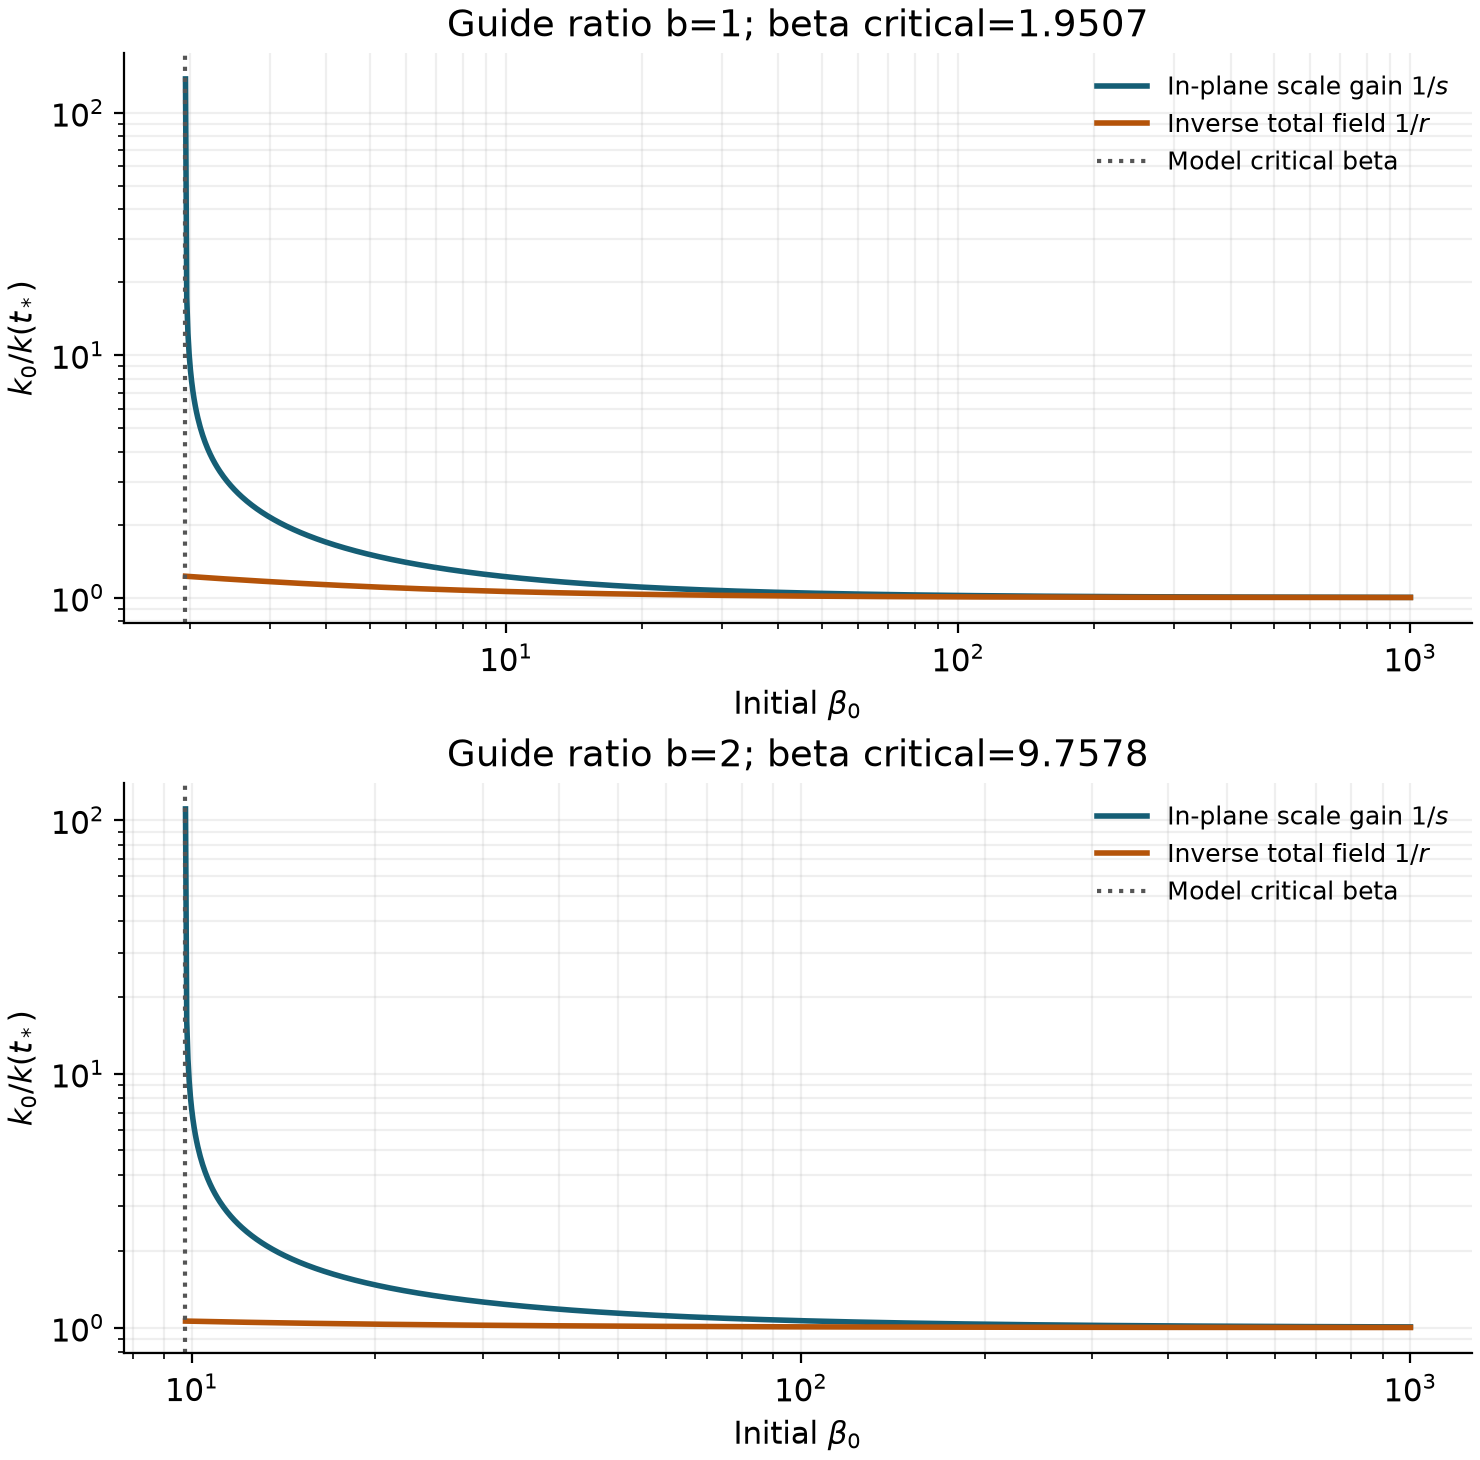
\includegraphics[keepaspectratio]{images/model-scale-conversion.png}}

Figure 1. Model scale conversion for \(b=1\) and \(b=2\). The source's
guide-field accessibility boundary remains unchanged. The divergent
corrected curve is limited physically by finite size and model
applicability, neither of which is imposed as an unmeasured numerical
cutoff here.

\pandocbounded{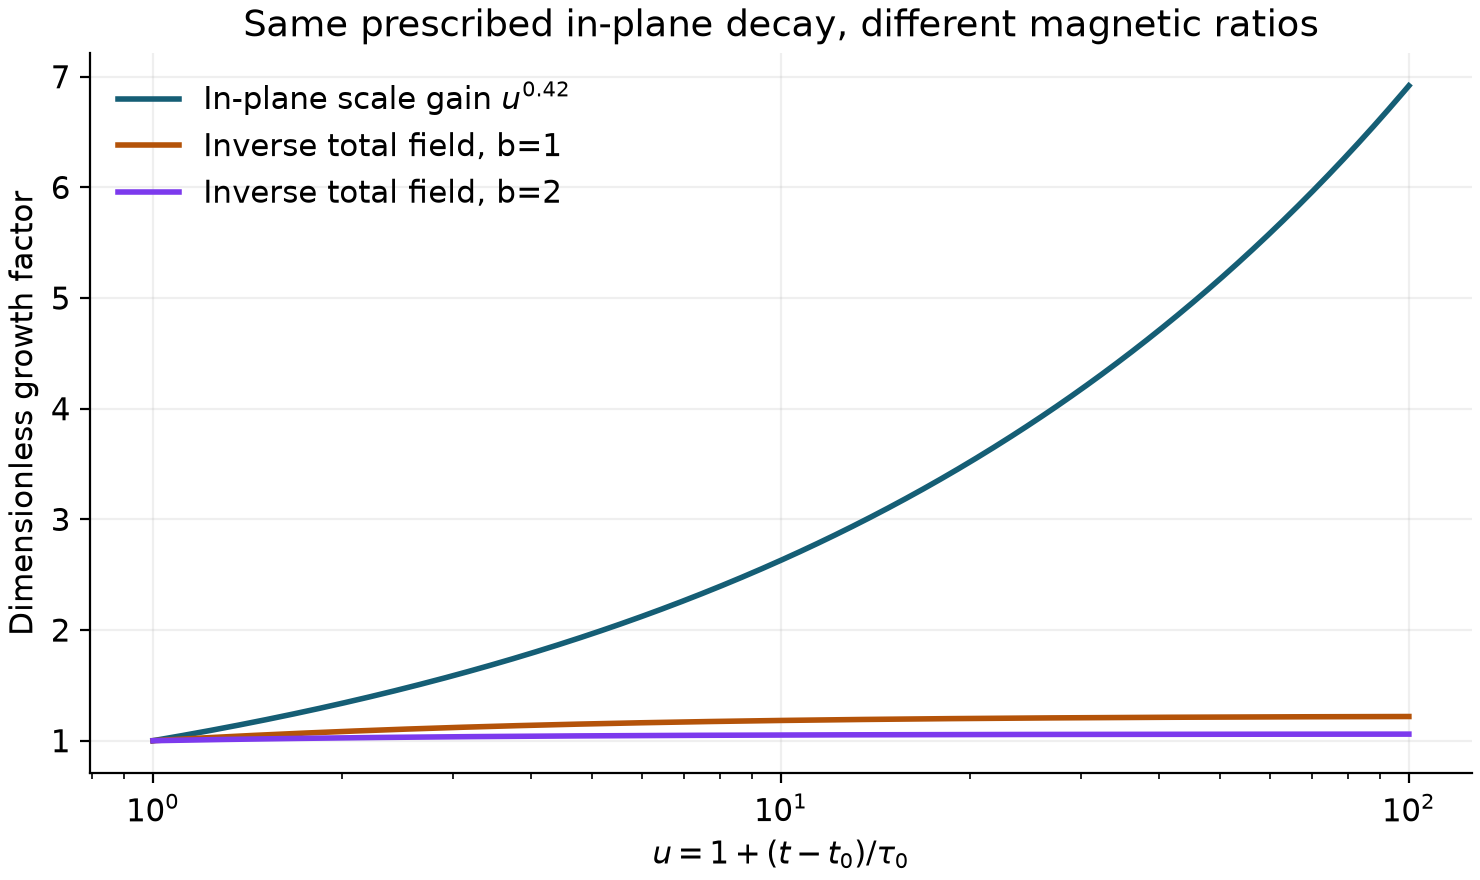
\includegraphics[keepaspectratio]{images/total-versus-in-plane.png}}

Figure 2. Ratio conversion for \(\alpha=0.42\). The horizontal
coordinate is the source's normalized time \(u\); no physical crossing
time or post-arrest evolution is fitted.

\subsection{4. Conditional numerical
checks}\label{conditional-numerical-checks}

The supplied reproduction solves Eq. (4) by monotone bisection and
independently checks its positive root using the full quartic
polynomial. It then evaluates the accessible root using Eq. (2).
Thirteen crossing cases include the zero-guide limit, both finite guide
ratios, inaccessible crossings, and successively closer approaches to
each critical beta. Separate temporal checks include the initial \(u=1\)
control. An inaccessible mathematical root is recorded with null
physical-branch gain and time rather than plotted as an allowed
crossing.


\begin{minipage}{\linewidth}\small
\begin{tabular}{@{}
  >{\raggedright\arraybackslash}p{(\linewidth - 8\tabcolsep) * \real{0.2000}}
  >{\raggedright\arraybackslash}p{(\linewidth - 8\tabcolsep) * \real{0.2000}}
  >{\raggedright\arraybackslash}p{(\linewidth - 8\tabcolsep) * \real{0.2000}}
  >{\raggedright\arraybackslash}p{(\linewidth - 8\tabcolsep) * \real{0.2000}}
  >{\raggedright\arraybackslash}p{(\linewidth - 8\tabcolsep) * \real{0.2000}}@{}}
\toprule\noalign{}
\begin{minipage}[b]{\linewidth}\raggedright
Guide ratio \(b\)
\end{minipage} & \begin{minipage}[b]{\linewidth}\raggedright
Initial \(\beta_0\)
\end{minipage} & \begin{minipage}[b]{\linewidth}\raggedright
Inverse total ratio \(1/r_*\)
\end{minipage} & \begin{minipage}[b]{\linewidth}\raggedright
In-plane gain \(K\)
\end{minipage} & \begin{minipage}[b]{\linewidth}\raggedright
Model crossing
\end{minipage} \\
\midrule\noalign{}
0 & 10.8 & 1.055368 & 1.055368 & Finite \\
1 & 3 & 1.163042 & 2.142550 & Finite \\
1 & 2 & 1.220744 & 8.726781 & Finite \\
2 & 10 & 1.059341 & 7.082716 & Finite \\
2 & 100 & 1.006580 & 1.064357 & Finite \\
2 & 1 & 1.353210 & Not accessible & None \\
\bottomrule\noalign{}
\end{tabular}
\end{minipage}


Table 1. Values of the stated analytic model, not corrected measurements
of simulation spectra. The zero-guide row is a formal algebraic control
outside the source's acknowledged CGL applicability near magnetic nulls.
The \(b=1\), \(\beta_0=3\) row uses the source's approximate initial
parameters as an illustration; its transient and imperfect averaged
closure still matter. The \(b=2\), \(\beta_0=1\) case demonstrates why
solving the scalar polynomial is insufficient without checking the
accessible field interval.

For \(b=1\), \(\beta_c=1.950734\); for \(b=2\), \(\beta_c=9.757772\).
The \(b=2\), \(\beta_0=10\) example shows that a large conversion
difference is not confined to a low-beta algebraic limit. It remains a
conditional closure calculation. It is not evidence that the physical
system actually reaches that growth, that its instability remains
unregulated, or that the observed spectral peak should be replaced by
the table entry.

An independent calculation uses 80-digit decimal arithmetic and a
separate equation in \(s^2\). Its total-field roots agree to about
\(1.2\times10^{-16}\) absolute. The closest critical cases amplify
floating-point cancellation in the converted gain, with a maximum
relative difference about \(1.2\times10^{-9}\). The six-decimal table
therefore avoids implying precision from the root residual alone.
Machine-readable outputs retain the unrounded values and the comparison
receipt.

The force-balance check in Section 5 is also exercised on a periodic
\(128^2\) grid using Fourier derivatives, with source-normalized
\(B_0=0.5\), \(T_0=0.25\), pair pressure \(2nT_0\) and four constant
guide amplitudes. Its maximum component residual is
\(1.40\times10^{-14}\) or smaller. A deliberately nonuniform added guide
produces a residual of 0.05. A separate analytic trigonometric
evaluation confirms both the unchanged constant-guide force balance and
the nonuniform negative control. This is a check of an initial field
identity; grid size here does not represent a new kinetic simulation.

All checks run locally without fetching source PDFs or executing unknown
source code. No particles are evolved, no dispersion solver is rerun and
no statistical confidence interval is attached to these deterministic
identities. The original source analysis scripts, simulation histories
and plotting chain have not been recovered through this calculation. The
illustrative clock uses \(\alpha=0.42\); the source reports different
fitted slopes in its guide cases. No guide-specific time history is
refitted here, and the root-to-scale algebra itself is independent of
\(\alpha\).

\subsubsection{Finite guide field in the journal's anisotropy-drive
estimate}\label{finite-guide-field-in-the-journals-anisotropy-drive-estimate}

The journal adds a kinetic-firehose growth calculation and a comparison
between instability growth and anisotropy drive {[}1,Section4,pp.4-5{]}.
The idea of comparing these actual times is sound. Its intermediate
assertion that every in-plane merger decreases \(Q=T_\perp/T_\parallel\)
by \(2^{-3/2}\), however, drops the constant guide contribution. Define
the modeled characteristic in-plane magnetic fraction

\[
\chi=\frac{B_{\rm in}^2}{B_{\rm in}^2+B_G^2}.
\]

The same approximately fixed-density CGL closure gives
\(Q\propto\mathcal B^3\). For one prescribed merger
\(B_{\rm in}\mapsto B_{\rm in}/\sqrt2\),

\[
\frac{Q_{\rm next}}{Q}
=\left(\frac{B_G^2+B_{\rm in}^2/2}{B_G^2+B_{\rm in}^2}\right)^{3/2}
=\left(1-\frac\chi2\right)^{3/2}.
\]

The source's factor follows only when \(\chi=1\). At its initial modeled
amplitude, \(\chi_0=1/(1+2b^2)\):


\begin{minipage}{\linewidth}\small
\begin{tabular}{@{}llll@{}}
\toprule\noalign{}
\(b\) & \(\chi_0\) & Guide-dependent \(Q_{\rm next}/Q\) & Printed
factor \\
\midrule\noalign{}
0 & 1 & 0.353553 & 0.353553 \\
1 & 1/3 & 0.760726 & 0.353553 \\
2 & 1/9 & 0.917835 & 0.353553 \\
\bottomrule\noalign{}
\end{tabular}
\end{minipage}


Table 2. A single modeled merger, holding the guide field constant. This
is a conditional temperature-ratio factor, not a fitted simulation
measurement. As the in-plane field decays, \(\chi\) also changes, so
successive identical in-plane reductions do not produce a constant
logarithmic decrement in \(Q\).

The corresponding differential relation is

\[
\frac{d\ln(1+\Delta)}{dt}
=3\chi\frac{d\ln B_{\rm in}}{dt}
=-\frac{3\alpha\chi}{\tau_0u}.
\]

With \(\tau_B=-(d\ln B_{\rm in}/dt)^{-1}\), a short interval near
isotropy and large parallel beta gives the local estimate

\[
t_{\rm cross}\simeq\frac{2\tau_B}{3\beta_\parallel\chi}.
\]

This approximation requires that beta, \(\chi\) and drive change little
over the crossing interval; initially it needs \(\beta_0\chi_0\gg1\). It
is not applicable to an arbitrarily delayed crossing near \(G=0\) and
does not replace the accessibility test. Under a constant fractional
in-plane decay, identifying a merger time with a factor-\(\sqrt2\)
reduction changes an order-one coefficient. It cannot remove a
parametrically small \(\chi\) from the drive.

A related normalization needs care in the reduction from journal Eq.(5)
to Eq.(6). The reconnection Alfvén speed is explicitly based on the
in-plane field, whereas beta, gyrofrequency and Larmor radius use the
total field. With consistent thermal and mass-density conventions, the
scaling is \(v_{\rm th}/v_{A,{\rm in}}\propto\sqrt{\beta/\chi}\), rather
than \(\sqrt\beta\). Combining this distinction with the local drive
factor yields a conditional growth-to-drive parameter proportional to
\((R/\rho)/(\beta\chi^{3/2})\), up to order-one constants and the
assumed reconnection rate. It does not justify a universal replacement
for Eq.(6): the actual distribution, growth rate and integrated drive
would still need evaluation. The reproduction separately checks the
exact generation factors and power-law derivative, leaving the original
dispersion solver and physical arrest untouched.

\subsection{5. Uniform-guide scalar-MHD force
balance}\label{uniform-guide-scalar-mhd-force-balance}

The journal attributes an early transient to the initial configuration
ceasing to be an exact MHD equilibrium when a guide field is included
{[}1, p.10{]}. That explanation conflicts with the stated field
geometry. This is a force-balance question independent of the averaged
CGL approximation.

Write the initial field as
\(\mathbf B_{\rm in}(x,y)+B_G\hat{\mathbf z}\), where \(B_G\) is
spatially uniform and the planar field has no z dependence. Ampère's law
then gives

\[
\mathbf J=\frac{c}{4\pi}\nabla\times\mathbf B_{\rm in}
=J_z(x,y)\hat{\mathbf z}.
\]

The added guide produces no current. Moreover,

\[
\frac{\mathbf J\times(\mathbf B_{\rm in}+B_G\hat{\mathbf z})}{c}
=\frac{\mathbf J\times\mathbf B_{\rm in}}{c},
\]

because parallel vectors have zero cross product. Therefore, if the
source's scalar pressure satisfies
\(\nabla p=\mathbf J\times\mathbf B_{\rm in}/c\) initially, the same
pressure satisfies force balance after adding any constant \(B_G\). This
argument preserves whatever force residual the planar configuration
already has; it does not require stability.

The explicit source profile confirms the result. With \(q=2\pi k_0/L\),
its fields are \(B_x=-B_0\cos(qx)\sin(qy)\) and
\(B_y=B_0\sin(qx)\cos(qy)\) {[}1, Section 2{]}. Their curl is solely out
of plane. Equivalently, a constant guide adds spatially constant
magnetic pressure and contributes no \((\mathbf B\cdot\nabla)\mathbf B\)
term in this two-dimensional geometry.

This correction does not eliminate the reported transient.
Scalar-pressure MHD balance is weaker than a stationary Vlasov
distribution: it does not specify particle orbits, pressure-tensor
evolution, discretization effects or relaxation. A guide field can alter
those processes while leaving the initial scalar-MHD force unchanged.
Identifying the actual cause would require kinetic initial-condition and
simulation diagnostics beyond the present calculation. The supported
conclusion is that the uniform guide alone cannot break the stated
scalar-MHD balance.

\subsection{6. Discussion}\label{discussion}

The main distinction is between the magnetic quantity that governs a
modeled instability and the quantity that defines a merger scale. The
guide field belongs in the total amplitude used by the source's
anisotropy closure. It cannot be left inside a field-to-size conversion
derived for the decaying reconnecting component. Equations (1)-(7) make
that separation explicit while retaining the source's scalar firehose
equation. The same distinction gives the finite-guide generation factor
and susceptibility in Section 4; dropping it also makes the simplified
anisotropy-drive estimate guide independent.

The published Fig. 7(b) is labeled as an inverse cascade ratio and is
discussed as evidence that growth remains small over a wide range of
beta {[}1{]}. The total-field proxy provides an artificial finite
plateau as the in-plane field declines. The corrected model gain has a
different behavior near its accessibility boundary. An analytic plot or
quantitative statement about merger-scale gain should therefore use Eq.
(2), identify its valid branch and explain the finite-box and closure
limits. A total-field amplification plot can still be useful if labeled
as that quantity.

This correction does not establish that the source's spectra or observed
arrest are wrong. The final article supplies local pressure-anisotropy
diagnostics, a kinetic growth calculation, and explicit applicability
caveats. Its kinetic-firehose competition is a stronger argument than
the preprint's earlier discussion, and the present deterministic checks
do not replace that calculation. The justified correction is to an
internal conversion and an equilibrium explanation, with any measured
change to the physical growth left for a matched simulation reanalysis.

\subsection{7. Limitations, reproducibility and
disclosures}\label{limitations-reproducibility-and-disclosures}

This audit is edition-specific. The supplied arXiv PDF and the authentic
journal version were read in full, with equations and decisive
paragraphs checked visually. Hashes, page locators and a substantive
concordance identify them. One provisional size-ratio observation in the
archived working concordance is excluded from the manuscript's findings
because geometric conventions remain unresolved;
\nolinkurl{SOURCE_SCOPE.md} documents that boundary. The comparison does
not claim a character-by-character editorial diff. Bounded correction
searches found no identified erratum; they do not prove that no
correction or inaccessible data deposit exists.

The main results are conditional on the source's own
characteristic-field prescription, averaged CGL closure and in-plane
merger scaling. The local kinetic invariants do not automatically imply
the chosen separate-average relations. Density changes, heat flux,
nonadiabatic motion, spatial intermittency and unstable fluctuations may
affect their accuracy. Near a critical curve, a formally large model
gain can reach the box scale or leave the closure's useful domain. No
physical divergence is asserted.

A uniform guide's preservation of scalar-MHD force balance does not
establish an exact Vlasov equilibrium, stability, or the absence of a
genuine startup transient. It identifies what the stated scalar-MHD
explanation cannot supply. Diagnosing the actual transient requires
additional particle distributions, initialization details or matched
numerical controls. The proof does not assign an undocumented numerical
cause.

\textbf{Code and data availability.} The original analytic checks,
deterministic JSON/CSV outputs, standalone independent verifiers,
original figures and source-edition records are archived as software
version 1.0.0 {[}6{]}, \url{https://doi.org/10.5281/zenodo.23779360} ,
direct record \url{https://zenodo.org/records/23779360} . The frozen
computational commit is
\nolinkurl{8ecf2c6407731de91025208153a269a59573e515} in
\url{https://github.com/Teylersf/inverse-transfer-guide-field-audit} .
Its 25-file ZIP contains 242,467 bytes, SHA-256
\nolinkurl{f0f4396b3f2d534683d16a9c42d373071c86943a9d0f6e086eff7ccc0c645214}.
A clean Git-tree extraction reproduced all four programs and preserved
all 25 file bytes in the recorded environment. Exact byte identity is
not promised for arbitrary platforms, library versions or fonts; the
independent numerical tolerances remain material.

On 29 October 2026, the anonymous Zenodo API and archive download
returned HTTP 200 with the expected creator, ORCID, software type,
version, commit and component licenses. The primary DataCite record,
\url{https://api.datacite.org/dois/10.5281/zenodo.23779360} , returned
HTTP 200 and state \nolinkurl{findable}; doi.org resolved to the public
Zenodo record and its registration-authority service confirmed DataCite.
\nolinkurl{submissions/zenodo-code-v1.0.0.json} retains timestamped
metadata and exact archive verification. The software DOI is distinct
from paper acceptance and need not appear in Crossref to be valid.

Source PDFs remain in a separate local cache, linked by their official
references rather than bundled as the author's work. Reproduction needs
no original HPC path, private data, GPU or new PIC run. Venue
submission, moderation, review and publication states are recorded
separately from these computational checks.

Taylor Kalin is the canonical author and self-funds this study. No
outside funding or competing interests have been reported. AI tools
assisted with retrieval, derivations, code, adversarial computational
checks and drafting. Those checks are not independent human peer review.
Any separately authorized agent-only edition identifies its agent author
and preserves Taylor Kalin's credit as human operator and canonical
author. The source authors and their institutions have not endorsed this
audit. Original audit code is MIT licensed; original text and figures
are CC BY 4.0. Attributed source material retains its own rights.

\subsection{8. Conclusion}\label{conclusion}

A finite uniform guide field separates total-field decay from the decay
of the reconnecting component. Within the source's stated model, the
in-plane scale gain is \([(1+2b^2)r_*^2-2b^2]^{-1/2}\), rather than
\(1/r_*\). The difference is quantitative and can become large near the
model boundary, although very-high-beta gains still approach one at
fixed guide ratio. The corrected conversion retains the scalar firehose
criterion and its accessible branch. The same field distinction supplies
a guide-dependent anisotropy generation factor and drive susceptibility;
its local timescale consequence is conditional and does not provide a
universal replacement arrest criterion. A missing factor of two in the
printed temporal exponent and an incorrect scalar-MHD explanation of the
startup transient are separate, localized corrections. None of these
identities alone supplies a corrected kinetic spectrum or overturns the
observed suppression mechanism.

\clearpage
\subsection{References}\label{references}

{[}1{]} Z. Liu, M. Zhou and N. F. Loureiro, \emph{Suppression of Inverse
Magnetic Energy Transfer in Collisionless Marginally Magnetized
Plasmas}, The Astrophysical Journal Letters \textbf{995}, L46 (2025).
\url{https://doi.org/10.3847/2041-8213/ae247e} . Version of record,
online 11 December 2025; issue date 20 December 2025.

{[}2{]} Z. Liu, M. Zhou and N. F. Loureiro, \emph{Suppression of inverse
magnetic energy transfer in collisionless marginally magnetized
plasmas}, arXiv:2510.01573v1 (2 October 2025).
\url{https://arxiv.org/abs/2510.01573v1} ;
\url{https://arxiv.org/pdf/2510.01573v1} . Earlier edition, identified
separately from {[}1{]}.

{[}3{]} G. F. Chew, M. L. Goldberger and F. E. Low, \emph{The Boltzmann
equation and the one-fluid hydromagnetic equations in the absence of
particle collisions}, Proceedings of the Royal Society of London A
\textbf{236}, 112-118 (1956).
\url{https://doi.org/10.1098/rspa.1956.0116} . Bibliographic metadata
verified directly; the closure as used here is explicitly stated in
{[}1{]}.

{[}4{]} M. Zhou, P. Bhat, N. F. Loureiro and D. A. Uzdensky,
\emph{Magnetic island merger as a mechanism for inverse magnetic energy
transfer}, Physical Review Research \textbf{1}, 012004(R) (2019).
\url{https://doi.org/10.1103/PhysRevResearch.1.012004} .

{[}5{]} M. Zhou, N. F. Loureiro and D. A. Uzdensky, \emph{Multi-scale
dynamics of magnetic flux tubes and inverse magnetic energy transfer},
Journal of Plasma Physics \textbf{86}, 535860401 (2020).
\url{https://doi.org/10.1017/S0022377820000641} .

{[}6{]} T. Kalin, \emph{Computational evidence for Guide-field
normalization and cascade growth in collisionless magnetic-island
merging}, version 1.0.0, Zenodo (2026), software and data.
\url{https://doi.org/10.5281/zenodo.23779360} . Computational snapshot
\nolinkurl{8ecf2c6407731de91025208153a269a59573e515}.
